% Cambio de base: las coordenadas son etiquetas
% Números y figuras PNG: apunte/scripts/cap09_cambio_de_base.py (uv run python apunte/scripts/cap09_cambio_de_base.py)
\chapter{Cambio de base: las coordenadas son etiquetas}\label{cap:cambio-base}

\section{La idea}

Un mojón está donde está. Sus coordenadas, en cambio, aparecen recién cuando elegimos con qué
medirlo: un par de números en la cuadrícula este--norte, otro en el sistema de la obra, otro en
el sistema local con que se orientó el instrumento. Este capítulo ordena qué cambia y qué no al
cambiar de base. Las coordenadas de un vector cambian con la \emph{inversa} de la matriz de
cambio; las filas (las formas lineales del capítulo~\ref{cap:formas-lineales}) cambian con la
matriz misma; la matriz de una transformación cambia por \emph{semejanza}. Lo que no cambia
---el valor de una forma sobre un vector, el determinante, la traza, los autovalores y, en bases
ortonormales, las longitudes--- es lo que tiene significado geométrico. Y la recompensa de
entenderlo es práctica: una transformación que en la grilla canónica no tiene lectura fácil, en
la grilla de sus autovectores es sólo estirar.

\paragraph{Convenciones del capítulo.} Vectores en columna. La base vieja es la canónica
\(e=(e_1,e_2)\) (o, en el campo, los ejes este y norte); la nueva es \(b=(b_1,\dots,b_n)\).
\([v]_e\) y \([v]_b\) son las coordenadas del mismo vector \(v\) en cada base, y
\(C=C_{b\to e}\) es la matriz de cambio de base (definición~\ref{def:matriz-cambio-base}).
Es la misma matriz que el recuadro de la sección~\ref{sec:cambio-base} llama \(P\); cuando la
base nueva es de autovectores, el párrafo del despeje la llama \(A\). Las tres letras designan
lo mismo: una matriz con la base nueva en columnas, que lleva de la base nueva a la vieja.

\subsection{El mismo vector con dos grillas}\label{sec:mismo-vector-dos-grillas}

En la figura~\ref{fig:cb-dos-grillas} la flecha violeta es una sola. En la grilla cuadrada
llegamos a su punta avanzando \(7\) pasos de \(e_1\) y \(4\) de \(e_2\): sus coordenadas son
\((7,4)\). En la grilla oblicua que generan \(b_1=(3,1)\) y \(b_2=(1,2)\) llegamos a la misma
punta con \(2\) pasos de \(b_1\) y \(1\) de \(b_2\), porque \(2(3,1)+1(1,2)=(7,4)\): sus
coordenadas son \((2,1)\). Ninguno de los dos pares es ``el verdadero''; cada uno es la
respuesta a la pregunta ``¿cuántos pasos de cada vector de la base?''.

\begin{figure}[htbp]
\centering
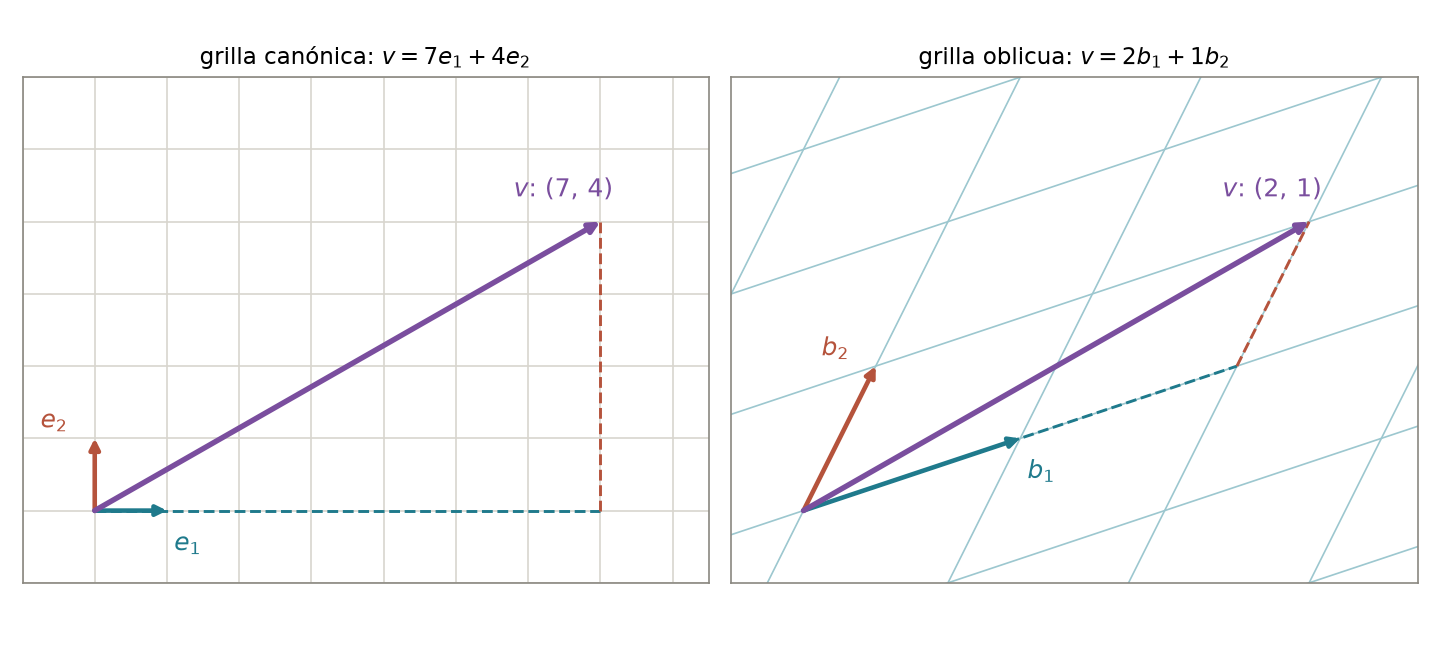
\includegraphics[width=.95\linewidth]{figuras/cambio-de-base/cb_dos_grillas.png}
\caption{El vector \(v\) es el mismo en los dos paneles. Izquierda: en la grilla canónica,
\(v=7e_1+4e_2\), coordenadas \((7,4)\). Derecha: en la grilla oblicua de \(b_1=(3,1)\) y
\(b_2=(1,2)\), \(v=2b_1+1b_2\), coordenadas \((2,1)\). Los tramos punteados son el camino de
lectura: tantos pasos del primer vector de la base, después tantos del segundo. Generada con
\texttt{apunte/scripts/cap09\_cambio\_de\_base.py}.}
\label{fig:cb-dos-grillas}
\end{figure}

La escalera de siempre ayuda a no perderse. En \(\R\) una base es un único vector, la unidad, y
cambiar de base es cambiar de unidad: si la unidad se hace cien veces más corta (de metros a
centímetros), el número se hace cien veces más grande. En \(\R^2\) la grilla puede, además,
inclinarse y tener pasos distintos en cada dirección. En \(\R^n\) la información del cambio
cabe en una matriz \(n\times n\) invertible. Lo que se repite en todos los escalones es el
sentido del cambio: si la base ``crece'', los números ``achican'', y viceversa.

\begin{idea}[El vector no se mueve: cambia la regla con que lo medimos]
Coordenadas y vector no son lo mismo. El vector es la flecha; las coordenadas son etiquetas
que dependen de la base elegida. Toda la técnica del capítulo consiste en traducir etiquetas
de una base a otra sin tocar la flecha, y en reconocer qué números no dependen de la
traducción.
\end{idea}

\unidadInteractiva{08_cambio_de_base}{Cambio de base y diagonalización}{Explorá: en el caso «base oblicua de la parcela» el mojón \(P=(4,3)\) tiene coordenadas \((1,1)\) en la base \(b_1=(3,1)\), \(b_2=(1,2)\); mové el giro y el largo de \(b_2\) y mirá cómo cambian los números mientras el mojón queda quieto.}

\section{Construcciones, cuentas y ejemplos}

Armamos la matriz de cambio de base, vemos cómo se transforman con ella las coordenadas, las
filas y las matrices, y la usamos para elegir la base en la que una transformación es más
simple.

\subsection{La matriz de cambio de base}\label{sec:matriz-cambio}

\begin{definicion}[Matriz de cambio de base]\label{def:matriz-cambio-base}
Sean \(e\) y \(b=(b_1,\dots,b_n)\) dos bases de \(\R^n\). La \emph{matriz de cambio de base}
\(C_{b\to e}\) es la matriz \(n\times n\) cuya columna \(j\) contiene las coordenadas de
\(b_j\) en la base \(e\):
\[
  C_{b\to e}=\bigl[\,[b_1]_e\ \big|\ [b_2]_e\ \big|\ \cdots\ \big|\ [b_n]_e\,\bigr].
\]
Es invertible porque sus columnas son linealmente independientes.
\end{definicion}

\begin{proposicion}[Las coordenadas cambian con la inversa]\label{prop:cb-coordenadas}
Para todo vector \(v\), con \(C=C_{b\to e}\),
\[
  [v]_e=C\,[v]_b,\qquad [v]_b=C^{-1}[v]_e .
\]
\end{proposicion}

\begin{demostracion}
Si \([v]_b=(c_1,\dots,c_n)\), entonces \(v=c_1b_1+\cdots+c_nb_n\). Tomando coordenadas en
\(e\), que es una operación lineal, \([v]_e=c_1[b_1]_e+\cdots+c_n[b_n]_e\), y una combinación
lineal de las columnas de \(C\) con coeficientes \(c_j\) es exactamente \(C\,(c_1,\dots,c_n)^T\).
Como \(C\) es invertible, se despeja \([v]_b=C^{-1}[v]_e\).
\end{demostracion}

El nombre \(C_{b\to e}\) dice qué hace la matriz: \emph{entran} coordenadas en \(b\) y
\emph{salen} coordenadas en \(e\). Para ir en el sentido que más se usa, de la base conocida a
la nueva, hay que invertir. Por eso se dice que las coordenadas son \emph{contravariantes}: la
base nueva se arma con \(C\) (sus vectores son las columnas) y las coordenadas pasan con
\(C^{-1}\), al revés. Las formas lineales, que son filas, pasan con \(C\) multiplicando a la
derecha, \([\varphi]_b=[\varphi]_e\,C\) (\emph{covariantes}; proposición~\ref{prop:co-contra}
del capítulo~\ref{cap:formas-lineales}), y así el número \(\varphi(v)\) no depende de la base.

\begin{ejemplo}[El mismo vector en dos bases, ida y vuelta]\label{ej:cb-oblicua}
Con \(b_1=(3,1)\) y \(b_2=(1,2)\), los de la figura~\ref{fig:cb-dos-grillas},
\[
  C=\begin{pmatrix}3&1\\1&2\end{pmatrix},\qquad \det C=5,\qquad
  C^{-1}=\frac15\begin{pmatrix}2&-1\\-1&3\end{pmatrix}.
\]
\emph{Ida.} Para \(v=(7,4)\),
\[
  [v]_b=C^{-1}\begin{pmatrix}7\\4\end{pmatrix}=\frac15\begin{pmatrix}14-4\\-7+12\end{pmatrix}
  =\begin{pmatrix}2\\1\end{pmatrix}.
\]
\emph{Vuelta.} \(C\,(2,1)^T=(6+1,\ 2+2)^T=(7,4)^T\): volvimos al punto de partida. La vuelta
es la cuenta fácil (multiplicar); la ida exige invertir o resolver un sistema.

\emph{Una forma lineal.} La forma \(\varphi=(1,1)\), que mide \(x+y\), vale
\(\varphi(v)=7+4=11\). En la base nueva su fila es \([\varphi]_b=(1,1)\,C=(3+1,\ 1+2)=(4,3)\):
sus componentes son \(\varphi(b_1)=4\) y \(\varphi(b_2)=3\). Con las coordenadas nuevas,
\((4,3)\cdot(2,1)=8+3=11\), el mismo número. Si por error se tratara a \(\varphi\) como un
vector y se la pasara con \(C^{-1}\), se obtendría \((0{,}2;\ 0{,}4)\), y el ``producto'' con
\((2,1)\) daría \(0{,}8\) en lugar de \(11\).
\end{ejemplo}

\subsection{La matriz de una transformación en otra base}\label{sec:semejanza}

Una transformación lineal \(T\) tampoco ``es'' una matriz: es una regla que lleva vectores en
vectores. Su matriz depende de la base en que se escriban los vectores que entran y los que
salen. Si en la base \(e\) la matriz es \(M_e\), ¿cuál es en la base \(b\)?

\begin{proposicion}[Matriz de una transformación en la base nueva]\label{prop:cb-semejanza}
Si \([Tv]_e=M_e\,[v]_e\) para todo \(v\) y \(C=C_{b\to e}\), entonces
\[
  [Tv]_b=M_b\,[v]_b\qquad\text{con}\qquad M_b=C^{-1}M_e\,C .
\]
Dos matrices relacionadas así se llaman \emph{semejantes}.
\end{proposicion}

\begin{demostracion}
Por la proposición~\ref{prop:cb-coordenadas},
\([Tv]_b=C^{-1}[Tv]_e=C^{-1}M_e[v]_e=C^{-1}M_e\,C\,[v]_b\).
\end{demostracion}

Se lee de derecha a izquierda, como un viaje: \(C\) traduce la entrada de \(b\) a \(e\),
\(M_e\) aplica la transformación donde sabemos escribirla, \(C^{-1}\) traduce la salida de
vuelta a \(b\). Lo que la matriz cambia es la descripción; la transformación es la misma, y
por eso hay números que no cambian.

\begin{proposicion}[Invariantes de semejanza]\label{prop:cb-invariantes}
Si \(M_b=C^{-1}M_eC\), entonces \(M_b\) y \(M_e\) tienen el mismo determinante, la misma traza
y el mismo polinomio característico; en particular, los mismos autovalores.
\end{proposicion}

\begin{demostracion}
\(\det M_b=\det C^{-1}\,\det M_e\,\det C=\det M_e\), porque \(\det C^{-1}=1/\det C\). Para la
traza se usa \(\operatorname{tr}(XY)=\operatorname{tr}(YX)\), que se verifica escribiendo las
dos sumas \(\sum_{i,k}X_{ik}Y_{ki}\): con \(X=C^{-1}\) e \(Y=M_eC\) queda
\(\operatorname{tr}M_b=\operatorname{tr}(M_eCC^{-1})=\operatorname{tr}M_e\). Para el
polinomio característico, \(M_b-\lambda I=C^{-1}(M_e-\lambda I)\,C\), y se toma determinante.
\end{demostracion}

Cada invariante tiene su hecho geométrico: el determinante es el factor de área con su signo
(capítulo~\ref{cap:subespacios}), que no puede depender de la grilla con que se midan las
áreas; los autovalores son los factores de estiramiento sobre las direcciones que no giran, y
una dirección que no gira lo hace en cualquier base; la traza es la suma de los autovalores.
Una entrada suelta de la matriz, en cambio, no significa nada por sí sola: cambia con la base.

\begin{ejemplo}[Reflexión respecto de una recta inclinada, por semejanza]\label{ej:cb-reflexion}
Queremos la matriz de la reflexión respecto de la recta \(y=x/2\), de dirección \((2,1)\).
Escribirla en la base canónica exige pensar; en una base adaptada a la recta es inmediata.
Tomamos \(b_1=(2,1)\), sobre la recta, y \(b_2=(-1,2)\), perpendicular a ella. La reflexión deja
quieto \(b_1\) y da vuelta \(b_2\): en la base \(b\) su matriz es \(\operatorname{diag}(1,-1)\).
Con
\[
  C=\begin{pmatrix}2&-1\\1&2\end{pmatrix},\qquad \det C=5,\qquad
  C^{-1}=\frac15\begin{pmatrix}2&1\\-1&2\end{pmatrix},
\]
la proposición~\ref{prop:cb-semejanza}, despejada para \(M_e\), da
\[
  M_e=C\begin{pmatrix}1&0\\0&-1\end{pmatrix}C^{-1}
  =\begin{pmatrix}2&1\\1&-2\end{pmatrix}\frac15\begin{pmatrix}2&1\\-1&2\end{pmatrix}
  =\frac15\begin{pmatrix}3&4\\4&-3\end{pmatrix}.
\]
Controles: \(M_e(2,1)^T=(2,1)^T\), \(M_e(-1,2)^T=(1,-2)^T\) y \(M_e(5,0)^T=(3,4)^T\), que tiene
el mismo largo \(5\). Invariantes: \(\det M_e=-1\), \(\operatorname{tr}M_e=0\), autovalores
\(1\) y \(-1\), los mismos que los de \(\operatorname{diag}(1,-1)\). La recta forma un ángulo
\(\alpha\approx26{,}5651^\circ\) con el eje \(x\), y \(\cos2\alpha=0{,}6\),
\(\sin2\alpha=0{,}8\): es la matriz \(H(\alpha)\) del capítulo~\ref{cap:reflexiones},
obtenida sin trigonometría. No hizo falta normalizar \(b_1\) y \(b_2\): \(C^{-1}\) absorbe los
largos. Con la base normalizada, \(U=C/\sqrt5\), vale \(U^{-1}=U^T\) y
\(U\operatorname{diag}(1,-1)U^T\) da la misma matriz (sección~\ref{sec:bases-ortonormales}).
\end{ejemplo}

\subsection{Diagonalizar: elegir la base en la que la transformación sólo estira}\label{sec:diagonalizar-base}

El ejemplo anterior sugiere la estrategia general. Si \(M\) tiene una base de autovectores
\(v_1,\dots,v_n\) con autovalores \(\lambda_1,\dots,\lambda_n\) (capítulo~\ref{cap:autovectores}),
en esa base la transformación manda cada \(v_j\) a \(\lambda_jv_j\): su matriz es diagonal.
Con la convención ya fijada en la sección~\ref{sec:cambio-base}, los autovectores van en las
columnas de \(A\), que lleva de la base de autovectores a la canónica, y
\[
  T_{\mathrm{can}}=A\,T_{\mathrm{diag}}\,A^{-1},\qquad
  T_{\mathrm{diag}}=A^{-1}\,T_{\mathrm{can}}\,A .
\]
Es la proposición~\ref{prop:cb-semejanza} con \(C=A\), \(M_e=T_{\mathrm{can}}\) y
\(M_b=T_{\mathrm{diag}}\). Diagonalizar es elegir la base en la que la transformación se ve
como escalas independientes sobre cada eje (figura~\ref{fig:cb-autovectores}). Las potencias
salen solas, porque los factores interiores se cancelan de a pares:
\[
  M^k=(ADA^{-1})(ADA^{-1})\cdots(ADA^{-1})=A\,D^k A^{-1},
\]
y \(D^k\) se calcula elevando cada entrada de la diagonal. Si los autovalores son positivos,
el exponente puede ser cualquier número real, \(M^t=AD^tA^{-1}\); en particular \(t=\tfrac12\)
da una raíz cuadrada de la matriz (sección~\ref{sec:raiz-matriz}).

\begin{figure}[htbp]
\centering
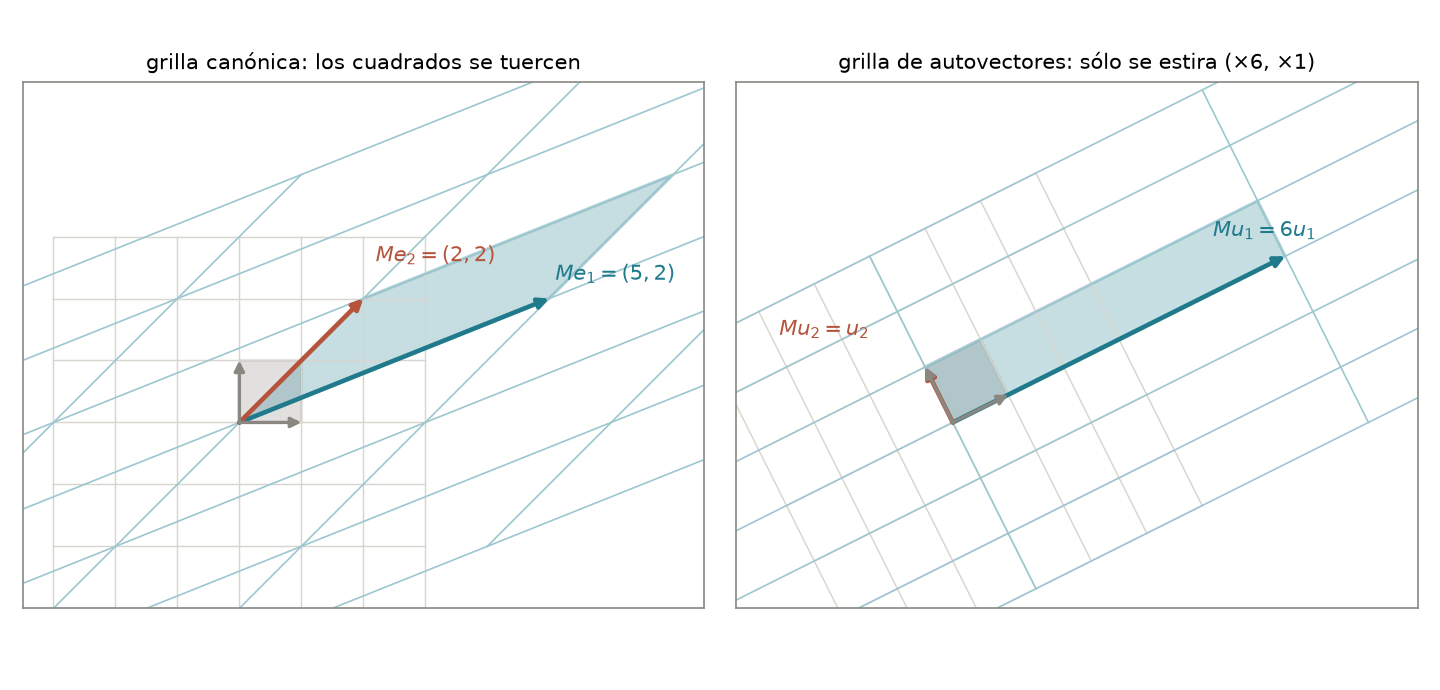
\includegraphics[width=.95\linewidth]{figuras/cambio-de-base/cb_autovectores.png}
\caption{La misma transformación \(M=\left(\begin{smallmatrix}5&2\\2&2\end{smallmatrix}\right)\)
aplicada a dos grillas (gris, antes; teal, después). Izquierda: la grilla canónica; el cuadrado
unidad se convierte en un paralelogramo torcido de lados \(Me_1=(5,2)\) y \(Me_2=(2,2)\).
Derecha: la grilla de los autovectores unitarios \(u_1=(2,1)/\sqrt5\), \(u_2=(-1,2)/\sqrt5\);
cada celda sólo se estira, \(\times6\) a lo largo de \(u_1\) y \(\times1\) a lo largo de
\(u_2\), y los ángulos rectos siguen rectos. Generada con
\texttt{apunte/scripts/cap09\_cambio\_de\_base.py}.}
\label{fig:cb-autovectores}
\end{figure}

\begin{ejemplo}[Diagonalizar una simétrica: \(M^{10}\) y \(M^{1/2}\)]\label{ej:cb-diagonalizar}
Sea \(M=\begin{pmatrix}5&2\\2&2\end{pmatrix}\). Su polinomio característico es
\(\lambda^2-7\lambda+6=(\lambda-6)(\lambda-1)\): autovalores \(6\) y \(1\) (control: suma
\(7=\operatorname{tr}M\), producto \(6=\det M\)). De \((M-6I)v=0\), es decir
\(-v_1+2v_2=0\), sale \(v_1=(2,1)\); de \((M-I)v=0\), es decir \(4v_1+2v_2=0\), sale
\(v_2=(-1,2)\). Son perpendiculares, como corresponde a una matriz simétrica. Con
\[
  A=\begin{pmatrix}2&-1\\1&2\end{pmatrix},\qquad
  A^{-1}=\frac15\begin{pmatrix}2&1\\-1&2\end{pmatrix},\qquad
  A^{-1}MA=\begin{pmatrix}6&0\\0&1\end{pmatrix}=D .
\]
(Es la misma \(A\) que la \(C\) del ejemplo~\ref{ej:cb-reflexion}: la reflexión respecto de
\(y=x/2\) y esta \(M\) son diagonales en la misma base.)

\emph{Potencia décima.} Con \(6^{10}=60\,466\,176\),
\[
  M^{10}=A\begin{pmatrix}6^{10}&0\\0&1\end{pmatrix}A^{-1}
  =\frac15\begin{pmatrix}4\cdot6^{10}+1&2\cdot6^{10}-2\\2\cdot6^{10}-2&6^{10}+4\end{pmatrix}
  =\begin{pmatrix}48\,372\,941&24\,186\,470\\24\,186\,470&12\,093\,236\end{pmatrix}.
\]
Multiplicar \(M\) por sí misma diez veces daría lo mismo con mucho más trabajo. Control por
invariantes: la traza es \(60\,466\,177=6^{10}+1^{10}\).

\emph{Raíz cuadrada.} Los autovalores son positivos; con \(\sqrt6\approx2{,}44949\),
\[
  M^{1/2}=A\begin{pmatrix}\sqrt6&0\\0&1\end{pmatrix}A^{-1}
  =\frac15\begin{pmatrix}4\sqrt6+1&2\sqrt6-2\\2\sqrt6-2&\sqrt6+4\end{pmatrix}
  \approx\begin{pmatrix}2{,}1596&0{,}5798\\0{,}5798&1{,}2899\end{pmatrix},
\]
y elevada al cuadrado devuelve \(M\) (el script lo verifica hasta el redondeo de máquina).
Hecho geométrico: \(M^{1/2}\) es ``la mitad del camino'': estira \(\sqrt6\approx2{,}449\) a lo
largo de \(v_1\) y deja quieto \(v_2\); aplicada dos veces, estira \(6\).
\end{ejemplo}

\subsection{Simulaciones}

\unidadInteractiva{08_cambio_de_base}{Cambio de base y diagonalización}{Verificá: elegí el caso «base de autovectores de A = [[2, 1], [1, 2]]» y comprobá que \(B^{-1}AB=\operatorname{diag}(3,1)\); después girá \(b_2\) con el deslizador y verificá que \(B^{-1}AB\) deja de ser diagonal pero la suma de su diagonal sigue valiendo \(4\): la traza no depende de la base.}

\section{En profundidad}

\subsection{Cambio de base y diagonalización}\label{sec:cambio-base}

{\small\vspace{1mm}\linkUnidad{08_cambio_de_base}{Simulación interactiva: Unidad 12 — Cambio de base y diagonalización}\par}
{\small\vspace{1mm}\linkAnimacion{03_cambio_de_base_viaje}{Animación: el viaje \(A\,T_{\mathrm{diag}}\,A^{-1}\)}\par}


El cambio de base y la diagonalización se desarrollan en el párrafo ``La matriz de cambio de
base y el despeje de la diagonalización''; después se extienden a potencias \(A^t\) y trayectorias.

\paragraph{Hecho geométrico: la flecha no se movió, cambió la grilla.} Un mojón tiene
coordenadas \((3,4)\) en la grilla cuadrada de siempre. Si en vez de los ejes canónicos usamos
las direcciones \(b_1=(1,1)\) y \(b_2=(1,-1)\), el \emph{mismo} punto se escribe
\[
  \begin{pmatrix}3\\4\end{pmatrix}
  =\tfrac72\begin{pmatrix}1\\1\end{pmatrix}-\tfrac12\begin{pmatrix}1\\-1\end{pmatrix},
  \qquad\text{coordenadas nuevas }(\tfrac72,-\tfrac12).
\]
El mojón está donde estaba; cambió la regla con que lo medimos. Escalera: en \(\R\) cambiar
de base es cambiar de unidad (de metros a centímetros el número se multiplica por 100 y la
longitud no cambia); en \(\R^2\) la grilla puede ser oblicua y con pasos distintos; en
\(\R^n\) es una matriz \(n\times n\) invertible. No parece
haber un conjunto de vectores privilegiado a priori: lo único que distingue a la base
canónica es que con ella el producto interno es la cuenta de siempre.

\begin{resultado}[La matriz de cambio de base]
Si \(P\) tiene en sus columnas los vectores de la base nueva escritos en la canónica,
\[
  [v]_{\text{can}}=P\,[v]_{\text{nueva}},\qquad [v]_{\text{nueva}}=P^{-1}[v]_{\text{can}} .
\]
Con \(P=\begin{pmatrix}1&1\\1&-1\end{pmatrix}\), \(P^{-1}=\tfrac12\begin{pmatrix}1&1\\1&-1\end{pmatrix}\)
y \(P^{-1}(3,4)^T=(\tfrac72,-\tfrac12)^T\), como arriba. Los tres tipos de objeto cambian
de base distinto, y conviene escribir siempre el sentido (acá, de la canónica a la nueva):
los vectores como \([v]_{\text{nueva}}=P^{-1}[v]_{\text{can}}\); las formas lineales, que
son filas, multiplicando por \(P\) del lado derecho, \([\varphi]_{\text{nueva}}=[\varphi]_{\text{can}}\,P\)
(sección~\ref{sec:formas-lineales}), para que \(\varphi(v)\) dé lo mismo en las dos bases;
y las transformaciones con
\[
  A_{\text{nueva}}=P^{-1}\,A\,P ,
\]
que se lee de derecha a izquierda: pasamos las coordenadas nuevas a canónicas, aplicamos \(A\)
como siempre, volvemos a las nuevas. Todo se convierte a la vez para que ninguna relación
cambie: cada punto sigue en su recta y \(A\) sigue llevando cada punto adonde lo llevaba.
\end{resultado}

\paragraph{Ejercicio resuelto: grilla de formas y vector.} Consigna: formas lineales \((1,1)\) y \((-1,2)\), vector \((3,4)\), transformación
\(T=\begin{pmatrix}1{,}2&0{,}5\\-0{,}1&1{,}3\end{pmatrix}\), elegida no muy distinta de
la identidad. Dibujar las curvas de nivel de las dos formas (dos mazos de rectas
paralelas que juntos arman una grilla), ubicar el vector en la grilla, transformar el
vector con \(T\) y las formas con \(T^{-1}\), redibujar y verificar que el vector
transformado cae en la misma intersección. Antes de transformar, \((1,1)\cdot(3,4)=7\) y
\((-1,2)\cdot(3,4)=5\): el vector está en la séptima curva de una y la quinta de la otra.
Inversa por adjunta sobre determinante, \(\det T=1{,}56+0{,}05=1{,}61\):
\[
  T^{-1}=\frac1{1{,}61}\begin{pmatrix}1{,}3&-0{,}5\\0{,}1&1{,}2\end{pmatrix},\qquad
  T\begin{pmatrix}3\\4\end{pmatrix}=\begin{pmatrix}5{,}6\\4{,}9\end{pmatrix},
\]
\[
  (1,1)\,T^{-1}=\tfrac1{1{,}61}(1{,}4,\ 0{,}7)=(0{,}870,\ 0{,}435),\qquad
  (-1,2)\,T^{-1}=\tfrac1{1{,}61}(-1{,}1,\ 2{,}9)=(-0{,}683,\ 1{,}801).
\]
Verificación: \(0{,}870\cdot5{,}6+0{,}435\cdot4{,}9=7{,}0\) y
\(-0{,}683\cdot5{,}6+1{,}801\cdot4{,}9=5{,}0\). El vector transformado sigue en la séptima
curva de la primera forma y en la quinta de la segunda. La forma \((1,1)\)
queda \((0{,}86,\ 0{,}43)\), se acuesta un poco (redondeo), y la \((-1,2)\) queda un poco más
vertical. Hecho geométrico: la grilla se deformó con el plano y el punto se movió con el
plano; medido con la grilla deformada, el punto está donde estaba. No hacemos nada: convertimos
todo para que nada cambie. En planilla: dos columnas
para la forma, dos para el vector, \texttt{SUMAPRODUCTO}.

\paragraph{Diagonalizar es elegir la grilla de los autovectores.} Sea
\(A=\begin{pmatrix}2&1\\1&2\end{pmatrix}\). Polinomio característico
\((2-\lambda)^2-1=0\), autovalores \(3\) y \(1\), autovectores \((1,1)\) y \((1,-1)\)
(perpendiculares porque \(A\) es simétrica). Con esos autovectores como columnas de \(P\),
\[
  P^{-1}AP=\tfrac12\begin{pmatrix}1&1\\1&-1\end{pmatrix}
  \begin{pmatrix}3&1\\3&-1\end{pmatrix}
  =\begin{pmatrix}3&0\\0&1\end{pmatrix}=D .
\]
Hecho geométrico: en la grilla de los autovectores la transformación es dos estiramientos
independientes, por \(3\) a lo largo de \(b_1\) y por \(1\) a lo largo de \(b_2\); la grilla
``se estira o se comprime pero no se rompe''. En la grilla común la misma transformación
no tiene lectura fácil. Equivale a aplicar dos afinidades
axiales sucesivas.

\paragraph{La matriz de cambio de base y el despeje de la diagonalización.} En este
párrafo usamos otros nombres: \(A\) es la matriz que tiene los autovectores en
columnas (la \(P\) del recuadro de arriba, con otro nombre) y \(T\) es la transformación
(la \(A\) del párrafo anterior).

\emph{El diagrama de conmutatividad.} Dualidad y cambio de base se juntan en una sola
cadena, escrita en orden de aplicación (de izquierda a derecha):
\[
  (p)\;\to\;(A)\;\to\;[\,A^{-1}\to T_{\mathrm{diag}}\to A\,]\;\to\;(A^{-1})\;\to\;(\ell) .
\]
En un extremo entra un punto \(p\) y en el otro una recta \(\ell\), los dos escritos en la
base de autovectores; lo que se mide es la incidencia. Con la convención de abajo (\(A\)
lleva de la base de autovectores a la canónica), el punto pasa a la canónica como \(A\,p\)
y la forma como \(\ell\,A^{-1}\) (multiplicando del lado derecho). El recuadro del medio
recibe y devuelve coordenadas canónicas: adentro actúa \(T_{\mathrm{diag}}\), en la base
de autovectores, y el recuadro entero, leído como producto (lo que se aplica último va a la
izquierda), es \(A\,T_{\mathrm{diag}}\,A^{-1}=T_{\mathrm{can}}\), la misma transformación
escrita en la base canónica. La cadena completa es
\(\ell A^{-1}\,(A\,T_{\mathrm{diag}}\,A^{-1})\,A\,p=\ell\,T_{\mathrm{diag}}\,p\): las
conversiones se absorben de a pares (\(A^{-1}A=I\)) y la incidencia no cambia; el punto
transformado sigue cayendo en la recta transformada. Despejar
\(T_{\mathrm{diag}}=A^{-1}\,T_{\mathrm{can}}\,A\) es sacar la diagonal del recuadro, como
hacemos más abajo. Todo se convierte a la vez para que nada cambie.

\emph{La matriz con los autovectores en columnas.} Definimos \(A=[\,v_1\mid v_2\,]\), los
autovectores escritos en la base canónica, uno por columna, y la probamos con el vector
\((1,0)^T\):
\[
  A\begin{pmatrix}1\\0\end{pmatrix}
  =\begin{pmatrix}A_{11}&A_{12}\\A_{21}&A_{22}\end{pmatrix}\begin{pmatrix}1\\0\end{pmatrix}
  =\begin{pmatrix}A_{11}\\A_{21}\end{pmatrix}=v_1 .
\]
Entra una unidad del primer autovector escrita en la base de autovectores y sale ese mismo
autovector escrito en la canónica: \(A\) traduce de la base de autovectores a la canónica
y \(A^{-1}\) hace el camino inverso, de la canónica a la de autovectores. El recorrido
completo para un punto cualquiera: el punto \((1,1)=e_x+e_y\), dado en la canónica, pasa
con \(A^{-1}\) a coordenadas \((c_1,c_2)\) en la base de autovectores, es decir
\((1,1)=c_1v_1+c_2v_2\); ahí la transformación es diagonal y devuelve
\((\lambda_1c_1,\ \lambda_2c_2)\); y \(A\) traduce ese resultado de vuelta a la canónica,
\(\lambda_1c_1v_1+\lambda_2c_2v_2\), que es \(T(1,1)\). Con la matriz del párrafo
anterior, \(v_1=(1,1)\) y \(v_2=(1,-1)\), el punto \((1,1)\) es el propio \(v_1\):
\((c_1,c_2)=(1,0)\), la diagonal da \((3,0)\) y \(A\) devuelve \(3v_1=(3,3)\), que
coincide con \(\begin{pmatrix}2&1\\1&2\end{pmatrix}(1,1)^T=(3,3)^T\).

\emph{El despeje.} El mismo recorrido, escrito como producto de matrices, dice que la
transformación en la base canónica es la diagonal conjugada por el cambio de base:
\[
  T_{\mathrm{can}}=A\,T_{\mathrm{diag}}\,A^{-1}
  \quad\Longrightarrow\quad
  T_{\mathrm{diag}}=A^{-1}\,T_{\mathrm{can}}\,A ,
\]
leída de derecha a izquierda: \(A^{-1}\) lleva a la base de autovectores,
\(T_{\mathrm{diag}}\) estira cada eje propio, \(A\) vuelve a la canónica. El despeje se
hace multiplicando por \(A^{-1}\) a la izquierda y por \(A\) a la derecha; los dos
productos \(A^{-1}A=I\) y \(A\,A^{-1}=I\) que aparecen se cancelan y queda
\(T_{\mathrm{diag}}\) sola. Con los nombres de este apunte (\(P\) para la matriz de
autovectores, \(A\) para la transformación) es exactamente el \(D=P^{-1}AP\) del párrafo
anterior: misma matriz, otro nombre.

\paragraph{Potencias y la trayectoria de un punto.} Volvemos a los nombres del apunte:
\(P\) es la matriz de autovectores y \(A\) la transformación. Como \(A=PDP^{-1}\),
\(A^n=PD^nP^{-1}\): aplicar \(n\) veces la transformación es estirar \(n\) veces cada eje
propio. Para \(n=5\),
\[
  A^5=P\begin{pmatrix}243&0\\0&1\end{pmatrix}P^{-1}
  =\tfrac12\begin{pmatrix}244&242\\242&244\end{pmatrix}
  =\begin{pmatrix}122&121\\121&122\end{pmatrix}.
\]
Lectura: \((1,0)=\tfrac12(1,1)+\tfrac12(1,-1)\); la parte en \((1,1)\) se multiplica por
\(243\) y la parte en \((1,-1)\) queda igual: \(\tfrac12(243,243)+\tfrac12(1,-1)=(122,121)\),
la primera columna. Si los autovalores son positivos el exponente puede ser real:
\(A^t=PD^tP^{-1}\) con \(D^t=\operatorname{diag}(3^t,1)\), y el punto \((1,0)\) recorre
\[
  A^t\begin{pmatrix}1\\0\end{pmatrix}=\tfrac12\begin{pmatrix}3^t+1\\3^t-1\end{pmatrix}:
  \quad(1,0)\ \text{en } t=0,\quad(1{,}37,\,0{,}37)\ \text{en } t=\tfrac12,\quad(2,1)\ \text{en } t=1 .
\]
Es la tercera idea del hilo (sección~\ref{sec:hilo}): la transformación se identifica con
la trayectoria que genera, y la potencia real la convierte en película. La misma jugada que
la exponencial de una rotación, ahora con estiramientos en vez de giros. La unidad
\texttt{08\_cambio\_de\_base} (apéndice~\ref{ap:notebooks}) tiene el deslizador en \(t\).

\paragraph{Dirección de cada cambio de base.} En la factorización \(A=P\,D\,P^{-1}\), el factor de la derecha, el que actúa primero sobre un vector en canónica, es el que \emph{convierte de la canónica a la base de autovectores}. Con subíndices descriptivos:
\(A\,T_{\mathrm{diag}\langle Av\rangle}A^{-1}=T_{\mathrm{no\,diag}\langle\mathrm{can}\rangle}\)
con \(A\) = autovectores en columnas, que es \(P\,D\,P^{-1}\) de arriba. Para no mezclar, en este apunte \(P\) siempre tiene la base nueva en columnas y se lee ``\(P\) lleva de la nueva a la canónica''.

\begin{resultado}[Diagonalizabilidad no tiene nada que ver con invertibilidad: cuatro matrices testigo]
Las dos preguntas, ``¿qué pasa si hay algo en el núcleo?'' y ``¿qué pasa si
un autovalor repetido no alcanza para armar una base?'', son independientes. Invertir
pide que el núcleo sea \(\{0\}\), es decir, que ningún autovalor sea \(0\). Diagonalizar
pide una base de \(\R^2\) formada por autovectores. Las cuatro combinaciones aparecen:
\medskip

\renewcommand{\arraystretch}{1.35}
\noindent\begin{tabular}{@{}p{2.6cm}p{1.1cm}p{2.2cm}p{2.1cm}p{5.6cm}@{}}
\textbf{Matriz} & \(\det\) & \textbf{Autovalores} & \textbf{¿Base de autovectores?} & \textbf{Hecho geométrico}\\
\hline
\textbf{1.}~\(\bigl(\begin{smallmatrix}2&0\\0&1\end{smallmatrix}\bigr)\) & \(2\ne0\) & \(2,\ 1\) & sí, \(e_1,e_2\) &
diagonalizable e invertible: estira el eje \(x\) al doble y deja fijo el \(y\); dos direcciones propias independientes.\\
\textbf{2.}~\(\bigl(\begin{smallmatrix}1&0\\0&0\end{smallmatrix}\bigr)\) & \(0\) & \(\lambda_1=1,\ \lambda_2=0\) & sí, \(e_1,e_2\) &
proyección sobre el eje \(x\): aplasta el eje \(y\) al origen, sin inversa, pero con base completa de autovectores.\\
\textbf{3a.}~\(\bigl(\begin{smallmatrix}1&1\\0&1\end{smallmatrix}\bigr)\) & \(1\) & \(1\) (doble) & no: sólo \(e_1\) &
corte: invertible, con inversa \(\bigl(\begin{smallmatrix}1&-1\\0&1\end{smallmatrix}\bigr)\); sólo el eje \(x\) queda fijo.\\
\textbf{3b.}~\(\bigl(\begin{smallmatrix}0&-1\\1&0\end{smallmatrix}\bigr)\) & \(1\) & \(\pm i\) & no en \(\R\) &
giro de \(90^\circ\): invertible, ninguna recta real queda fija.\\
\textbf{4.}~\(\bigl(\begin{smallmatrix}0&1\\0&0\end{smallmatrix}\bigr)\) & \(0\) & \(0\) (doble) & no: sólo \(e_1\) &
ni diagonalizable ni invertible: manda \(e_2\mapsto e_1\) y \(e_1\mapsto0\).\\
\end{tabular}
\renewcommand{\arraystretch}{1.18}
\medskip

\textbf{Matriz 2.} Tener autovalor \(0\) impide invertir (el núcleo es el eje \(y\),
\(\det=0\)) y no impide diagonalizar: \(e_1\) y \(e_2\) son autovectores con
\(\lambda_1=1\), \(\lambda_2=0\), y en esa base la matriz ya es diagonal.

\textbf{Matriz 3a.} El polinomio característico es \((\lambda-1)^2=0\): la raíz
\(\lambda=1\) tiene multiplicidad algebraica \(2\). Pero \((A-I)v=0\) da \(v_2=0\), de modo
que el autoespacio es sólo el eje \(x\): multiplicidad geométrica \(1\). Falta un segundo
autovector, y sin él no hay base.

\textbf{Matriz 3b.} En el giro el motivo es otro: no hay rectas reales fijas, los
autovalores \(\pm i\) no son reales.

\textbf{Matriz 4.} \(\lambda=0\) doble, pero el núcleo es sólo el eje \(x\): un único
autovector \(e_1\).

El defecto de las matrices 3a, 3b y 4 es exactamente por lo que la sección~\ref{sec:svd}
pasa a la SVD, \(A=U\Sigma V^T\): con una base ortonormal a la entrada (\(V\)) y otra
\emph{distinta} a la salida (\(U\)), toda matriz, incluso un corte o una rectangular, se
lee como diagonal. Es diagonal entre dos grillas distintas, no una semejanza: \(\Sigma\) no
es ``\(A\) en otra base'', los \(\sigma\) no son autovalores (en el corte,
\(\sigma=(\sqrt5\pm1)/2\) y \(\lambda=1\) doble) y no sirve para potencias,
\(A^n\neq U\Sigma^nV^T\). Las dos descomposiciones coinciden sólo si \(A\) es simétrica
semidefinida positiva.
\linkUnidad{09_cambio_de_base_svd}{Simulación interactiva: cambio de base y SVD}
\end{resultado}

\subsection{Potencias reales y raíz cuadrada de una matriz}\label{sec:raiz-matriz}

La cuenta \(M^t=AD^tA^{-1}\) del ejemplo~\ref{ej:cb-diagonalizar} merece una afirmación
precisa, porque ``la raíz de una matriz'' no es ``la raíz de cada entrada''.

\begin{proposicion}[Raíz cuadrada de una matriz diagonalizable con autovalores positivos]\label{prop:cb-raiz}
Sea \(M=ADA^{-1}\) con \(D=\operatorname{diag}(\lambda_1,\dots,\lambda_n)\) y todos los
\(\lambda_j>0\). La matriz \(R=A\,D^{1/2}A^{-1}\), con
\(D^{1/2}=\operatorname{diag}(\sqrt{\lambda_1},\dots,\sqrt{\lambda_n})\), cumple \(R^2=M\),
tiene los mismos autovectores que \(M\) y autovalores \(\sqrt{\lambda_j}>0\). Si además \(A\)
tiene columnas ortonormales (como ocurre para \(M\) simétrica), \(R\) es simétrica.
\end{proposicion}

\begin{demostracion}
\(R^2=AD^{1/2}A^{-1}AD^{1/2}A^{-1}=A\,(D^{1/2})^2A^{-1}=ADA^{-1}=M\). Como \(v_j\) es la
columna \(j\) de \(A\), \(A^{-1}v_j=e_j\), y entonces
\(Rv_j=AD^{1/2}e_j=A\sqrt{\lambda_j}\,e_j=\sqrt{\lambda_j}\,v_j\). Si \(A^{-1}=A^T\),
\(R^T=(A^{-1})^TD^{1/2}A^T=AD^{1/2}A^{-1}=R\).
\end{demostracion}

No es la única matriz cuyo cuadrado es \(M\): cambiando el signo de alguna \(\sqrt{\lambda_j}\)
se obtienen otras (el ejercicio~\ref{ex:cb-raiz} muestra una). La de la proposición es la que
tiene todos los autovalores positivos, y es la que se usa cuando se habla de \emph{la} raíz.
Lo mismo vale para cualquier exponente real: \(M^t=AD^tA^{-1}\) cumple \(M^sM^t=M^{s+t}\), y
\(t\mapsto M^t\) interpola entre la identidad (\(t=0\)) y \(M\) (\(t=1\)), estirando cada eje
propio por \(\lambda_j^t\). Es la película del párrafo ``Potencias y la trayectoria de un
punto'', ahora con su justificación. Con un autovalor negativo la cuenta se rompe ya en
\(t=\tfrac12\): una reflexión no tiene raíz cuadrada real que estire cada eje propio, porque
\(\sqrt{-1}\) no es real.

\subsection{Bases ortonormales: \texorpdfstring{\(C^{-1}=C^T\)}{C inversa = C traspuesta}}\label{sec:bases-ortonormales}

Hasta acá todas las bases fueron igualmente buenas. El producto interno rompe esa igualdad.

\begin{proposicion}[Cambio entre bases ortonormales]\label{prop:cb-ortonormal}
Las columnas de \(C\) forman una base ortonormal si y sólo si \(C^TC=I\), es decir,
\(C^{-1}=C^T\). En ese caso:
\begin{enumerate}
  \item las coordenadas nuevas son productos internos, \([v]_b=C^T[v]_e\), o sea
  \(([v]_b)_j=b_j\cdot v\);
  \item el producto interno se calcula con la misma fórmula en las dos bases:
  \([u]_b\cdot[v]_b=[u]_e\cdot[v]_e\); en particular, las longitudes no cambian.
\end{enumerate}
\end{proposicion}

\begin{demostracion}
La entrada \((i,j)\) de \(C^TC\) es el producto interno de la columna \(i\) con la columna
\(j\), \(b_i\cdot b_j\); que valga \(1\) si \(i=j\) y \(0\) si no es la definición de base
ortonormal. Entonces \([v]_b=C^{-1}[v]_e=C^T[v]_e\), cuya entrada \(j\) es \(b_j\cdot v\). Y
\([u]_e\cdot[v]_e=(C[u]_b)^T(C[v]_b)=[u]_b^T\,C^TC\,[v]_b=[u]_b\cdot[v]_b\).
\end{demostracion}

\paragraph{Por qué estas bases son privilegiadas.} En una base cualquiera el producto interno
también se puede calcular, pero no con la cuenta de siempre: la misma demostración da
\(u\cdot v=[u]_b^T\,G\,[v]_b\) con \(G=C^TC\), la matriz de los productos \(b_i\cdot b_j\)
(matriz de Gram). En la base oblicua del ejemplo~\ref{ej:cb-oblicua},
\(G=\left(\begin{smallmatrix}10&5\\5&5\end{smallmatrix}\right)\), y para \(v=(7,4)\), con
\([v]_b=(2,1)\),
\[
  [v]_b^T\,G\,[v]_b=10\cdot2^2+2\cdot5\cdot2\cdot1+5\cdot1^2=65=7^2+4^2 ,
\]
mientras que la cuenta ingenua \(2^2+1^2=5\) no mide nada. El producto interno no elige
\emph{una} base: elige la familia de las bases con \(G=I\), y dos bases de esa familia difieren
en una matriz ortogonal (un giro o una reflexión, capítulo~\ref{cap:reflexiones}). En esas
bases desaparece, en la cuenta, la diferencia entre vectores y filas: las coordenadas pasan
con \(C^{-1}=C^T\) y la fila traspuesta pasa con \(C^T\), la misma matriz. Por eso, en una base
ortonormal, el gradiente se puede dibujar como una flecha sin cometer error
(sección~\ref{sec:formas-metrica}); en una base oblicua, no. Y por eso conviene diagonalizar
las matrices simétricas con autovectores \emph{normalizados}: son perpendiculares (lo
afirma el teorema espectral, que usamos sin demostración; en el
ejemplo~\ref{ej:cb-diagonalizar} se ve directamente), y con \(U=A/\sqrt5\) queda
\(M=U\,D\,U^T\), sin inversas que calcular.

\subsection{Lectura activa y lectura pasiva}\label{sec:activa-pasiva-cb}

La misma matriz admite dos lecturas, como ya vimos con las rotaciones
(definición de transformación activa y pasiva en la sección~\ref{sec:punto-coordenadas}).
Leída \emph{activamente}, \(C\) mueve vectores: manda \(e_j\) a \(b_j\). Leída
\emph{pasivamente}, \(C\) no mueve nada: traduce las etiquetas de un vector fijo de la base
\(b\) a la base \(e\). Girar el objeto un ángulo y girar los ejes el mismo ángulo producen
números que se relacionan por la matriz inversa (figura~\ref{fig:cb-activa-pasiva}).

\begin{figure}[htbp]
\centering
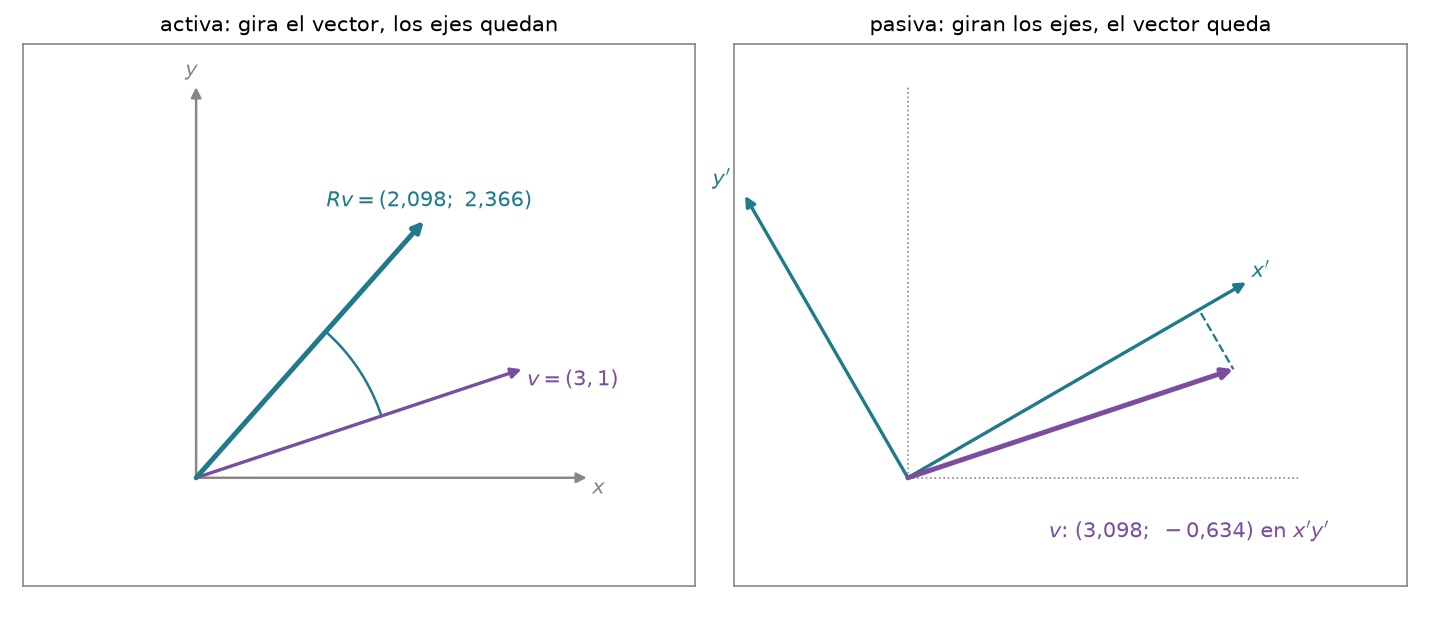
\includegraphics[width=.95\linewidth]{figuras/cambio-de-base/cb_activa_pasiva.png}
\caption{El vector \(v=(3,1)\) y un giro de \(30^\circ\). Izquierda (activa): los ejes quedan
y el vector gira; sus nuevas coordenadas son \(Rv\approx(2{,}098;\ 2{,}366)\). Derecha
(pasiva): el vector queda y giran los ejes; en los ejes nuevos el mismo vector tiene
coordenadas \(R^Tv\approx(3{,}098;\ -0{,}634)\). Generada con
\texttt{apunte/scripts/cap09\_cambio\_de\_base.py}.}
\label{fig:cb-activa-pasiva}
\end{figure}

\begin{ejemplo}[Girar el vector o girar los ejes]\label{ej:cb-activa-pasiva}
Sea \(v=(3,1)\) y \(R=R(30^\circ)\). \emph{Activa}: el vector girado tiene coordenadas
\(Rv=(3\cos30^\circ-\sin30^\circ,\ 3\sin30^\circ+\cos30^\circ)\approx(2{,}098;\ 2{,}366)\) en
los ejes de siempre. \emph{Pasiva}: los ejes nuevos son las columnas de \(R\), así que
\(C=R\) y, como la base es ortonormal, \([v]_b=R^Tv=(3\cos30^\circ+\sin30^\circ,\
-3\sin30^\circ+\cos30^\circ)\approx(3{,}098;\ -0{,}634)\). Las dos cuentas usan matrices
inversas entre sí, \(R(30^\circ)\) y \(R(-30^\circ)\); el módulo es \(\sqrt{10}\approx3{,}162\)
en los tres casos. Girar los ejes \(30^\circ\) produce las mismas etiquetas que girar el vector
\(-30^\circ\): por eso, ante una fórmula de cambio de coordenadas, la primera pregunta es
siempre qué se movió.
\end{ejemplo}

La semejanza \(M_b=C^{-1}M_eC\) también tiene sus dos lecturas. Pasiva: es la misma
transformación descripta en otra base. Activa: si \(C\) se piensa como un movimiento que lleva
la figura canónica a la figura \(b\), entonces \(CM_bC^{-1}=M_e\) es ``transportar la
transformación'': llevar el objeto a la posición estándar, transformar ahí y volver. Es
exactamente lo que se hizo en el ejemplo~\ref{ej:cb-reflexion}: la reflexión respecto de una
recta inclinada es la reflexión respecto del eje \(x\), transportada.

\subsection{Aplicación topográfica: coordenadas de obra}\label{sec:aplicacion-obra}

En una obra lineal (una vía, un canal, un camino) lo que importa de un corrimiento no son sus
componentes este y norte, sino cuánto se corrió \emph{a lo largo} del eje y cuánto \emph{hacia
un costado}. Un riel que se desplaza unos milímetros en la dirección de la vía casi no importa;
el mismo desplazamiento hacia el costado puede sacarlo de trocha. La herramienta es un cambio
a una base ortonormal adaptada al eje.

\paragraph{La base de obra.} El eje tiene acimut \(\mathrm{Az}=127^\circ30'\). Con \(E\) y \(N\)
como primera y segunda coordenada, la dirección de acimut \(\mathrm{Az}\) es
\((\sin\mathrm{Az},\ \cos\mathrm{Az})\) (sección~\ref{sec:acimut-campo}). Definimos
\(u_L\) según el eje y \(u_T\) a su derecha, es decir, con acimut \(\mathrm{Az}+90^\circ\):
\[
  u_L\approx(0{,}7934;\ -0{,}6088),\qquad u_T\approx(-0{,}6088;\ -0{,}7934),\qquad
  C=[\,u_L\mid u_T\,]\approx\begin{pmatrix}0{,}7934&-0{,}6088\\-0{,}6088&-0{,}7934\end{pmatrix}.
\]
\(C^TC=I\): la base es ortonormal y \(C^{-1}=C^T\). Además \(\det C=-1\): el par
(longitudinal, transversal a la derecha) gira en sentido horario, como los acimutes, al revés
que el par (este, norte). No es un problema: la proposición~\ref{prop:cb-ortonormal} sólo pide
columnas ortonormales. (En este caso \(C\) resulta además simétrica, de modo que
\(C^{-1}=C^T=C\): es una reflexión.)

\paragraph{Los datos.} Tres puntos de control materializados sobre el eje, en las progresivas
\(0\), \(100\) y \(200\) m, se midieron en dos campañas. Coordenadas Gauss-Krüger, faja 5, en
metros:

\begin{center}
\small
\begin{tabular}{crrrrrr}
\toprule
punto & \(E\) (1) & \(N\) (1) & \(E\) (2) & \(N\) (2) & \(\Delta E\) (mm) & \(\Delta N\) (mm)\\
\midrule
\(P_1\) & \(5\,512\,340{,}215\) & \(6\,178\,905{,}480\) & \(5\,512\,340{,}223\) & \(6\,178\,905{,}470\) & \(8\) & \(-10\)\\
\(P_2\) & \(5\,512\,419{,}550\) & \(6\,178\,844{,}604\) & \(5\,512\,419{,}557\) & \(6\,178\,844{,}606\) & \(7\) & \(2\)\\
\(P_3\) & \(5\,512\,498{,}886\) & \(6\,178\,783{,}728\) & \(5\,512\,498{,}871\) & \(6\,178\,783{,}737\) & \(-15\) & \(9\)\\
\bottomrule
\end{tabular}
\end{center}

Control de que los puntos están sobre el eje: \(P_2-P_1=(79{,}335;\ -60{,}876)\) m tiene
componente longitudinal \(100{,}0\) m y transversal \(0{,}0\) m; \(P_3-P_1\), \(200{,}0\) y
\(0{,}0\) m.

\paragraph{Desplazamientos en la base de obra.} Con \(d=(\Delta E,\Delta N)\) en mm, las
componentes de obra son \((d_L,d_T)=C^Td\): \(d_L=u_L\cdot d\), \(d_T=u_T\cdot d\). Por
ejemplo, para \(P_1\), \(d_L=0{,}7934\cdot8+(-0{,}6088)(-10)\approx12{,}43\) mm y
\(d_T=(-0{,}6088)\cdot8+(-0{,}7934)(-10)\approx3{,}06\) mm.

\begin{center}
\small
\begin{tabular}{crrrrr}
\toprule
punto & \((\Delta E,\Delta N)\) & \((d_L,d_T)\) & \(\lvert d\rvert\) en \(E,N\) & \(\lvert d\rvert\) en \(L,T\) & lectura\\
\midrule
\(P_1\) & \((8;\ -10)\) & \((12{,}43;\ 3{,}06)\) & \(12{,}81\) & \(12{,}81\) & avanza y se corre a la derecha\\
\(P_2\) & \((7;\ 2)\) & \((4{,}34;\ -5{,}85)\) & \(7{,}28\) & \(7{,}28\) & se corre a la izquierda\\
\(P_3\) & \((-15;\ 9)\) & \((-17{,}38;\ 1{,}99)\) & \(17{,}49\) & \(17{,}49\) & retrocede sobre el eje\\
\bottomrule
\end{tabular}
\end{center}

Los módulos coinciden en las dos bases, como asegura la proposición~\ref{prop:cb-ortonormal}:
cambiar a una base ortonormal reparte el mismo desplazamiento entre otras dos componentes, sin
agrandarlo ni achicarlo.

\paragraph{Una tolerancia que depende de la dirección.} Supongamos que el pliego admite
\(20\) mm de corrimiento longitudinal pero sólo \(5\) mm transversal. La región admisible es la
elipse de semiejes \(20\) mm según \(u_L\) y \(5\) mm según \(u_T\)
(figura~\ref{fig:cb-obra}), que en la base de obra es la curva de nivel \(1\) de la forma
cuadrática (capítulo~\ref{cap:svd})
\[
  q(d)=\frac{d_L^2}{20^2}+\frac{d_T^2}{5^2}=[d]_{LT}^T\,D\,[d]_{LT},\qquad
  D=\operatorname{diag}\Bigl(\frac1{400},\ \frac1{25}\Bigr)\ \text{mm}^{-2}.
\]
Un punto está dentro de tolerancia si \(q(d)\le1\). Para usarla directamente con
\(\Delta E,\Delta N\) hay que reescribir la matriz en la base \(E,N\). Como
\([d]_{LT}=C^T[d]_{EN}\), queda \(q=[d]_{EN}^T\,(C\,D\,C^T)\,[d]_{EN}\):
\[
  Q=C\,D\,C^T\approx10^{-3}\begin{pmatrix}16{,}397&18{,}111\\18{,}111&26{,}103\end{pmatrix}\ \text{mm}^{-2}.
\]
En una base cualquiera una forma cuadrática no cambia por semejanza sino con
\(Q=(C^{-1})^T D\,C^{-1}\) (sale de reemplazar \([d]_{LT}=C^{-1}[d]_{EN}\)); como esta base es
ortonormal, \(C^{-1}=C^T\) y las dos reglas coinciden: \(Q=C\,D\,C^{-1}\) es también la
semejanza de la proposición~\ref{prop:cb-semejanza}, y valen sus invariantes. Controles:
\(\operatorname{tr}Q=0{,}0425=\tfrac1{400}+\tfrac1{25}\) y \(\det Q=10^{-4}=\tfrac1{400\cdot25}\).
El término cruzado \(18{,}111\cdot10^{-3}\) aparece porque los ejes de la elipse no son los
ejes \(E,N\).

\begin{figure}[htbp]
\centering
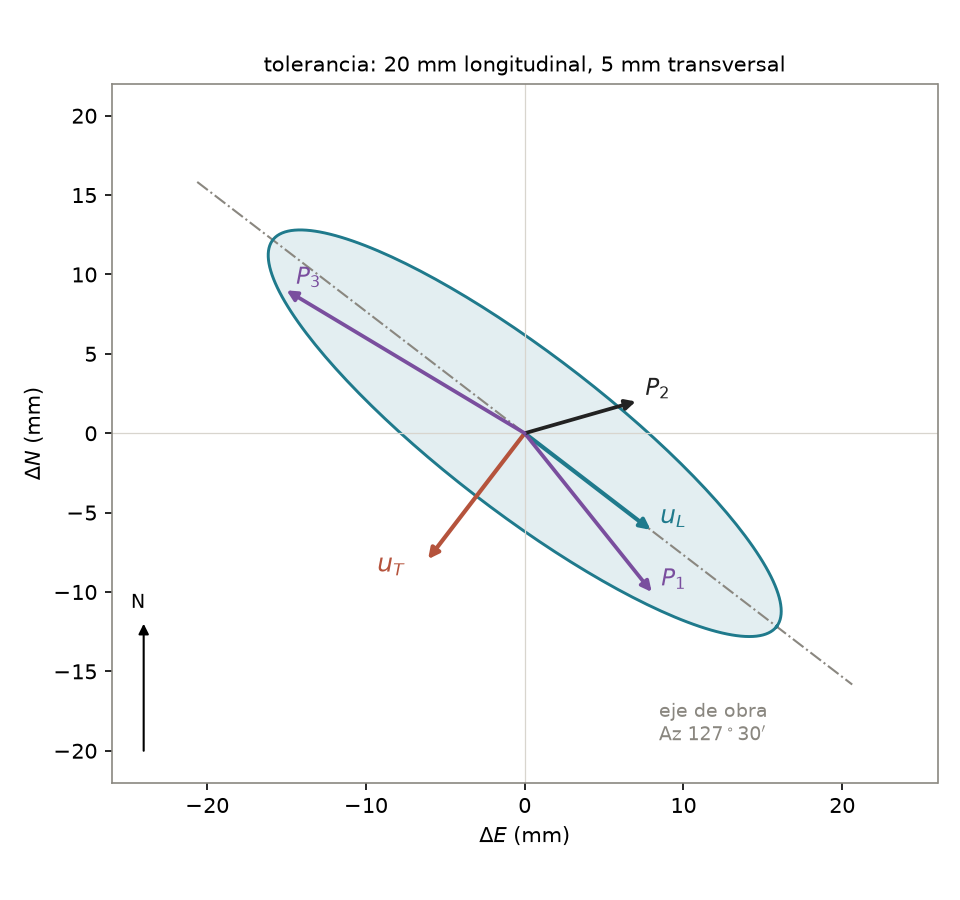
\includegraphics[width=.62\linewidth]{figuras/cambio-de-base/cb_obra.png}
\caption{Desplazamientos de los tres puntos de control, en mm, con la elipse de tolerancia de
semiejes \(20\) mm según el eje de obra (acimut \(127^\circ30'\)) y \(5\) mm hacia los
costados. \(P_1\) y \(P_3\) quedan dentro; \(P_2\), el desplazamiento más corto, queda fuera
porque es casi todo transversal. Generada con
\texttt{apunte/scripts/cap09\_cambio\_de\_base.py}.}
\label{fig:cb-obra}
\end{figure}

\paragraph{La decisión, en las dos bases.} Para \(P_2\), en la base de obra,
\(q=4{,}34^2/400+(-5{,}85)^2/25\approx0{,}0470+1{,}3680=1{,}4150\). En la base \(E,N\), con
\(d=(7,2)\),
\[
  q=10^{-3}\bigl(16{,}397\cdot7^2+2\cdot18{,}111\cdot7\cdot2+26{,}103\cdot2^2\bigr)
  \approx0{,}8035+0{,}5071+0{,}1044=1{,}4150 .
\]
El mismo número, como debía ser: \(q\) es una función del desplazamiento, no de sus etiquetas.
Para los tres puntos:

\begin{center}
\small
\begin{tabular}{crrrrc}
\toprule
punto & \(d_L^2/400\) & \(d_T^2/25\) & \(q\) en \(L,T\) & \(q\) en \(E,N\) & ¿\(q\le1\)?\\
\midrule
\(P_1\) & \(0{,}3865\) & \(0{,}3754\) & \(0{,}7619\) & \(0{,}7619\) & dentro\\
\(P_2\) & \(0{,}0470\) & \(1{,}3680\) & \(1{,}4150\) & \(1{,}4150\) & fuera\\
\(P_3\) & \(0{,}7551\) & \(0{,}1586\) & \(0{,}9137\) & \(0{,}9137\) & dentro\\
\bottomrule
\end{tabular}
\end{center}

La lectura es la que motivó el cambio de base. \(P_2\) tiene el desplazamiento más chico
(\(7{,}28\) mm) y es el único fuera de tolerancia, porque casi todo su corrimiento es
transversal; \(P_3\) se movió \(17{,}49\) mm y está dentro, porque se movió a lo largo del
eje. Una tolerancia circular de \(20\) mm habría aprobado los tres
(\(\lvert d\rvert/20=0{,}640\), \(0{,}364\) y \(0{,}875\)). En la base de obra la cuenta es
evidente; en la base \(E,N\) es la misma cuenta, con un término cruzado que la esconde.

\section{Ejercicios con solución}

\begin{ejercicio}\label{ex:cb-coordenadas}
Sea la base \(b_1=(1,1)\), \(b_2=(-1,2)\). (a) Escribir \(C=C_{b\to e}\) y \(C^{-1}\).
(b) Hallar las coordenadas de \(v=(1,7)\) en la base \(b\) y verificar volviendo a la canónica.
(c) Escribir en la base \(b\) la forma lineal \(\varphi=(2,-1)\) y comprobar que \(\varphi(v)\)
da lo mismo en las dos bases.
\end{ejercicio}
\solucion{(a) \(C=\left(\begin{smallmatrix}1&-1\\1&2\end{smallmatrix}\right)\), \(\det C=3\),
\(C^{-1}=\tfrac13\left(\begin{smallmatrix}2&1\\-1&1\end{smallmatrix}\right)\).
(b) \([v]_b=C^{-1}(1,7)^T=\tfrac13(2+7,\ -1+7)^T=(3,2)^T\); control
\(3(1,1)+2(-1,2)=(1,7)\). (c) \([\varphi]_b=(2,-1)\,C=(2-1,\ -2-2)=(1,-4)\). En la canónica,
\(\varphi(v)=2-7=-5\); en la base \(b\), \((1,-4)\cdot(3,2)=3-8=-5\).}

\begin{ejercicio}\label{ex:cb-proyeccion}
Obtener por semejanza, a partir de \(\operatorname{diag}(1,0)\), la matriz de la proyección
ortogonal sobre la recta de dirección \((3,4)\). Verificar que \(P^2=P\), calcular la imagen de
\((5,0)\) y de \((-4,3)\), y comparar determinante y traza con los de \(\operatorname{diag}(1,0)\).
\end{ejercicio}
\solucion{Base ortonormal adaptada: \(u=(3,4)/5\) sobre la recta, \(n=(-4,3)/5\) perpendicular;
en ella la proyección deja \(u\) y anula \(n\), matriz \(\operatorname{diag}(1,0)\). Con
\(U=[\,u\mid n\,]\), \(U^{-1}=U^T\) y
\(P=U\operatorname{diag}(1,0)\,U^T=uu^T=\tfrac1{25}\left(\begin{smallmatrix}9&12\\12&16\end{smallmatrix}\right)\).
\(P^2=P\) (proyectar dos veces es proyectar una). \(P(5,0)^T=(1{,}8;\ 2{,}4)^T\), sobre la
recta; \(P(-4,3)^T=(0,0)^T\), porque \((-4,3)\) es perpendicular. \(\det P=0\) y
\(\operatorname{tr}P=1\), iguales a los de \(\operatorname{diag}(1,0)\): autovalores \(1\) y
\(0\).}

\begin{ejercicio}\label{ex:cb-potencia}
Sea \(M=\begin{pmatrix}4&1\\2&3\end{pmatrix}\). (a) Hallar sus autovalores y autovectores.
(b) Calcular \(M^3\) como \(AD^3A^{-1}\). (c) ¿Es \(A^{-1}=A^T\)? ¿Por qué?
\end{ejercicio}
\solucion{(a) \(\lambda^2-7\lambda+10=(\lambda-5)(\lambda-2)\): autovalores \(5\) y \(2\)
(suma \(7=\operatorname{tr}M\), producto \(10=\det M\)). \(M(1,1)^T=(5,5)^T\) y
\(M(1,-2)^T=(2,-4)^T\): autovectores \((1,1)\) y \((1,-2)\).
(b) \(A=\left(\begin{smallmatrix}1&1\\1&-2\end{smallmatrix}\right)\), \(\det A=-3\),
\(A^{-1}=\tfrac13\left(\begin{smallmatrix}2&1\\1&-1\end{smallmatrix}\right)\),
\(M^3=A\operatorname{diag}(125,8)\,A^{-1}=\left(\begin{smallmatrix}86&39\\78&47\end{smallmatrix}\right)\),
lo mismo que multiplicando directamente; traza \(133=125+8\).
(c) No: \(A^TA=\left(\begin{smallmatrix}2&-1\\-1&5\end{smallmatrix}\right)\neq I\). Los
autovectores no son perpendiculares (\((1,1)\cdot(1,-2)=-1\)) porque \(M\) no es simétrica, y
ni normalizándolos se obtiene una base ortonormal.}

\begin{ejercicio}\label{ex:cb-raiz}
Hallar la raíz cuadrada con autovalores positivos de \(M=\begin{pmatrix}10&6\\6&10\end{pmatrix}\)
y verificarla. Encontrar otra matriz cuyo cuadrado también sea \(M\).
\end{ejercicio}
\solucion{Autovalores \(16\) y \(4\), con autovectores \((1,1)\) y \((1,-1)\). Con
\(A=\left(\begin{smallmatrix}1&1\\1&-1\end{smallmatrix}\right)\),
\(R=A\operatorname{diag}(4,2)\,A^{-1}=\left(\begin{smallmatrix}3&1\\1&3\end{smallmatrix}\right)\),
y \(R^2=\left(\begin{smallmatrix}9+1&3+3\\3+3&1+9\end{smallmatrix}\right)=M\). Cambiando el signo
de la primera raíz, \(A\operatorname{diag}(-4,2)\,A^{-1}=\left(\begin{smallmatrix}-1&-3\\-3&-1\end{smallmatrix}\right)\),
que también eleva al cuadrado a \(M\) pero tiene un autovalor negativo; la raíz de la
proposición~\ref{prop:cb-raiz} es \(R\).}
